\section{Прямые на плоскости}

\subsection{Векторное параметрическое уравнение прямой}

Пусть на плоскости задана система координат O, $\overline{e_1}$, $\overline{e_2}$.

\begin{wrapfigure}{l}{0.4\textwidth}
	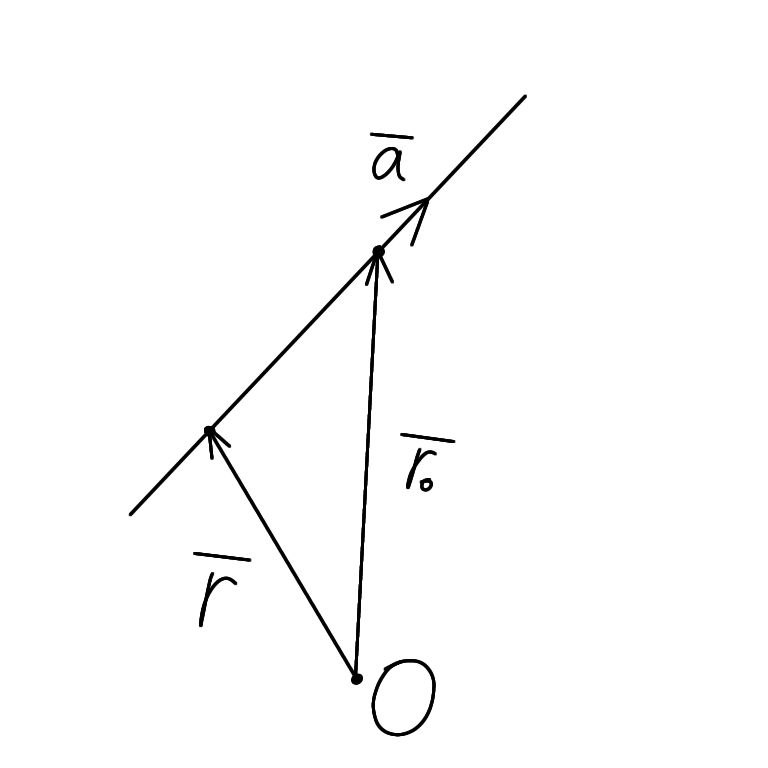
\includegraphics[width=0.84\linewidth]{images/1.1.jpeg}
\end{wrapfigure}

\tab\\
$\overline{a} \neq \overline{0}$ $-$ направляющий вектор\\

\underline{\textit{Векторное параметрическое уравнение прямой:}}
\[
\overline{r} = \overline{r_0} + \overline{a}t, t\in\R
\]
\[
\begin{pmatrix}
    x\\
    y\\
\end{pmatrix} = 
\begin{pmatrix}
    x_0\\
    y_0\\
\end{pmatrix} + 
\begin{pmatrix}
    a_x\\
    a_y\\
\end{pmatrix}t
\]
\tab\ \tab\\ \tab\\ \tab\\

\subsection{Общее уравнение прямой}

\begin{theorem}
    Любая прямая на плоскости может быть задана $\underline{\text{общим уравнением прямой}}$:
    \[
    Ax + By + C = 0, A^2 + B^2 > 0
    \]
\end{theorem}
\begin{proof}
    Точка $\overline{r}$ лежит на прямой тогда и только тогда, когда $\overline{r}$ - $\overline{r_0}$ и $\overline{a}$ $-$ коллинеарны, т.е.
    \[
    \begin{vmatrix}
        x - x_0 & y - y_0\\
        a_x & a_y\\
    \end{vmatrix} = 0
    \]
    \[
    \Longleftrightarrow
    \]
    \[
    a_y(x - x_0) - a_x(y-y_0) = 0
    \]
    \[
    \Longleftrightarrow
    \]
    \[
    a_y x - a_x y +(a_x y_0 - a_y x_0) = 0,
    \]
    \tab\\
    где $a_y$ = A, $- a_x$ = B, $a_x y_0 - a_y x_0$ = C
\end{proof}

\begin{corollary}
    В любой системе координат направляющий вектор прямой может быть выбран как (B, -A).
\end{corollary}

\begin{theorem}
    Если существует общее уравнение прямой, то оно задает прямую в любой системе координат.
\end{theorem}
\begin{proof}
    Рассмотрим точку ($x_0$, $y_0$), такую что
    \[
    Ax_0 + By_0 + C = 0
    \]
    Рассмотрим прямую, проходящую через точку ($x_0$, $y_0$), с направляющим вектором (В, -А). Подставив данные в векторное параметрическое уравнение прямой, получим искомое уравнение.
\end{proof}

\begin{theorem}
    Два уравнения задают одну прямую
    \[
    \begin{cases}
        A_1 x + B_1 y + C_1 = 0\\
        A_2 x + B_2 y + C_2 = 0\\
    \end{cases} \Longleftrightarrow \exists\lambda\neq 0 : A_1 = \lambda A_2, B_1 = \lambda B_2, C_1 = \lambda C_2
    \]
\end{theorem}
\begin{proof}
    \tab\\
    $\tab\Longleftarrow$\\
    Пусть $A_1 = \lambda A_2, B_1 = \lambda B_2, C_1 = \lambda C_2, \lambda\neq 0$. Подставим в общее уравнение прямой:
    \[
    A_1 x + B_1 y + C_1 = \lambda A_2 x + \lambda B_2 y + \lambda C_2 = \lambda(A_2 x + B_2 y + C_2) = 0,
    \]
    а т.к. $\lambda\neq 0$, получаем
    \[
    \begin{cases}
        A_1 x + B_1 y + C_1 = 0\\
        A_2 x + B_2 y + C_2 = 0\\
    \end{cases} - \text{одна прямая}
    \]

    $\tab\Longrightarrow$\\
    Т.к. заданные уравнения задают одну прямую, их направляющие векторы ($B_1$, -$A_1$) и ($B_2$, -$A_2$) $-$ коллинеарны $\Longrightarrow$ $\exists\lambda\neq 0$ : $A_1 = \lambda A_2, B_1 = \lambda B_2$, значит, чтобы уравнения были равносильны, необходимое условие: $C_1 = \lambda C_2$
\end{proof}

\subsection{Каноническое уравнение прямой}

Пусть задано 2 точки $\overline{r_1}$ и $\overline{r_2}$, значит направляющий вектор $\overline{a} = \overline{r_2} - \overline{r_1}$ $\Longrightarrow$
\[
\overline{r} = \overline{r_1} + t(\overline{r_2} - \overline{r_1})
\]
$-$ $\underline{\text{уравнение прямой через пару точек}}$.\\

Распишем координаты векторов.
\[
\begin{cases}
    x = x_0 + a_x t\\
    y = y_0 + a_y t\\
\end{cases} \Longrightarrow \dfrac{x - x_0}{a_x} = \dfrac{y - y_0}{a_y}
\]
Получили $\underline{\text{каноническое уравнение прямой}}$, причем при записи допускается, что $a_x$ или $a_y$ = 0. В таком случае задается прямая, параллельная одной из осей координат.\\

Аналогично для двух заданных точек $\overline{r_1}(x_1, y_1)$ и $\overline{r_2}(x_2, y_2)$:
\[
\dfrac{x - x_1}{x_2 - x_1} = \dfrac{y - y_1}{y_2 - y_1}
\]

\begin{corollary}
    Если задано каноническое уравнение прямой, то в знаменателях дробей стоят соответствующие координаты направляющего вектора. Это верно в любой системе координат.
\end{corollary}

\subsection{Уравнение прямой через нормальный вектор}

Если задать на прямой точку, ненулевой нормальный вектор $\overline{n}$ к этой прямой, то эта прямая задается однозначно.

\begin{wrapfigure}{l}{0.4\textwidth}
	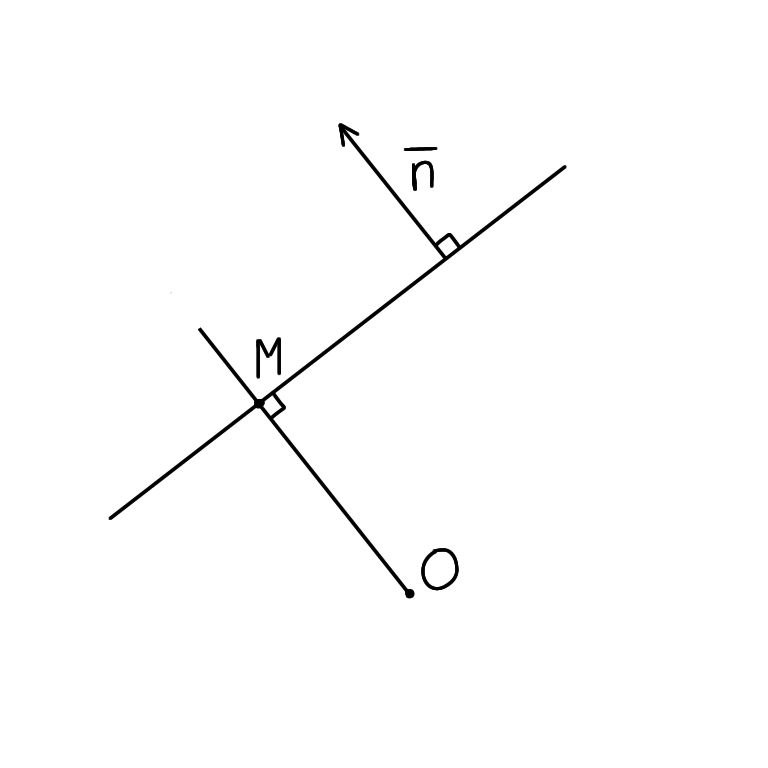
\includegraphics[width=0.84\linewidth]{images/1.2.jpeg}
\end{wrapfigure}

\tab\\

\[
(\overline{r} - \overline{r_0}, \overline{n}) = 0 \Longleftrightarrow (\overline{r}, \overline{n}) = (\overline{r_0}, \overline{n}) = d
\]

\[
\overline{r_M} = k\overline{n}, k = \dfrac{d}{(\overline{n}, \overline{n})}
\]

\[
\Longrightarrow \overline{r_M} = \dfrac{d}{(\overline{n}, \overline{n})}\overline{n}
\]

\tab\\
\textbf{В ОНБ.} 

\[
(\overline{r}, \overline{n}) = d, \text{где } \overline{r}(x, y), \overline{n}(n_x, n_y) \Longrightarrow n_x x + n_y y = d \Longrightarrow
\] если в ОНБ задано общее уравнение прямой, то вектор (А, В) $-$ один из нормальных векторов.

\subsection{Расстояние от точки до прямой}

\underline{В произвольной системе координат.}\\

Пусть заданы точка M : $\overline{r_1}$ и прямая l : ($\overline{r}$ - $\overline{r_0}$, $\overline{n}$) = 0.

\begin{wrapfigure}{l}{0.4\textwidth}
	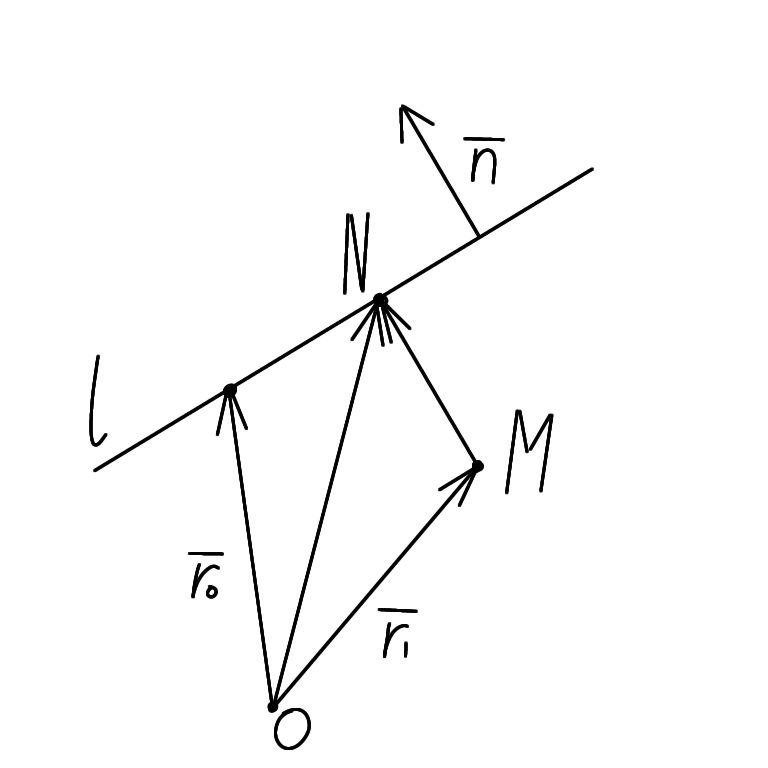
\includegraphics[width=0.84\linewidth]{images/1.3.jpeg}
\end{wrapfigure}

\tab\\

Тогда расстояние от точки М до прямой l \\
$\rho$ = |$\overline{MN}$|, $\overline{MN}$ = k$\overline{n}$

Мы знаем, что $\overline{ON}$ $-$ радиус-вектор точки, принадлежащей l $\Longrightarrow$ 

\[
(\overline{r_1} + k\overline{n} - \overline{r_0}, \overline{n}) = 0, k = \dfrac{(\overline{r_0} - \overline{r_1}, \overline{n})}{(\overline{n}, \overline{n})} \Longrightarrow
\]
\[
|\overline{MN}| = k\overline{n} = \dfrac{|(\overline{r_0} - \overline{r_1}, \overline{n})|}{|\overline{n}|} = |(\overline{r_0} - \overline{r_1}, \dfrac{\overline{n}}{|\overline{n}|})|
\]

\tab\\

\underline{В ОНБ.}\\

Пусть заданы точка М($x_1$, $y_1$) и прямая l : Ax + By + C = 0. Тогда в ОНБ расстояние от точки до прямой вычисляется как:
\[
\rho = \dfrac{|Ax_1 + By_1 + C|}{\sqrt{A^2 + B^2}}
\]

В любой системе координат прямая разбивает плоскость на 2 полуплоскости. Допустим, существует точка, лежащая вне прямой. Подставим эту точку в уравнение прямой, тогда в одной полуплоскости получим отрицательное значение, а в другой положительное.

\begin{wrapfigure}{l}{0.4\textwidth}
	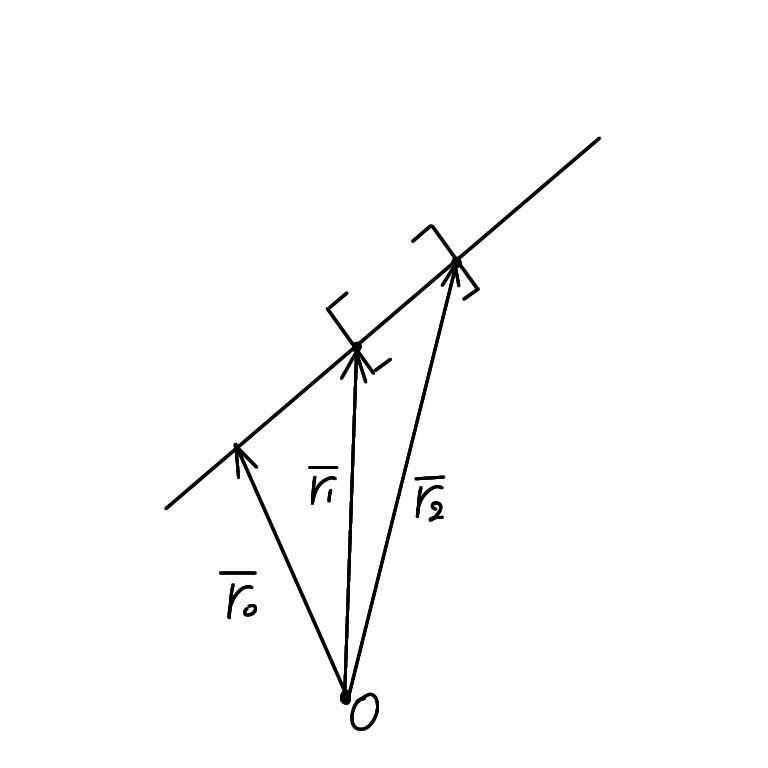
\includegraphics[width=0.84\linewidth]{images/1.4.jpeg}
\end{wrapfigure}

\tab\\

Чтобы задать отрезок на прямой, необходимо задать точки его концов
\[
\overline{r} = \overline{r_0} + t\overline{a}, t\in[t_1, t_2]
\]

\tab\\ \tab\\ \tab\\ \tab\\ \tab\\

\subsection{Пучок прямых}

\begin{definition}
    \textit{Пучок прямых} $-$ множество всех прямых, проходящих через заданную фиксированную точку.
\end{definition}

\begin{theorem}
    Пусть даны прямые
    \[
    \begin{cases}
        A_1 x + B_1 y + C_1 = 0\\
        A_2 x + B_2 y + C_2 = 0\\
    \end{cases} - \text{пересекающиеся} \Longrightarrow \text{пучок}.
    \] тогда
    \begin{enumerate}
        \item Для любой прямой пучка $\exists\alpha, \beta, \alpha^2 + \beta^2 > 0$ :
        \[
        \alpha(A_1 x + B_1 y + C_1) + \beta(A_2 x + B_2 y + C_2) = 0 - \text{уравнение этой прямой.}
        \]
        \item $\forall\alpha,\beta$, $\alpha^2 + \beta^2 > 0$:
        \[
        \alpha(A_1 x + B_1 y + C_1) + \beta(A_2 x + B_2 y + C_2) = 0 - \text{уравнение какой-то прямой из пучка.}
        \]
    \end{enumerate}
\end{theorem}
\begin{wrapfigure}{l}{0.4\textwidth}
    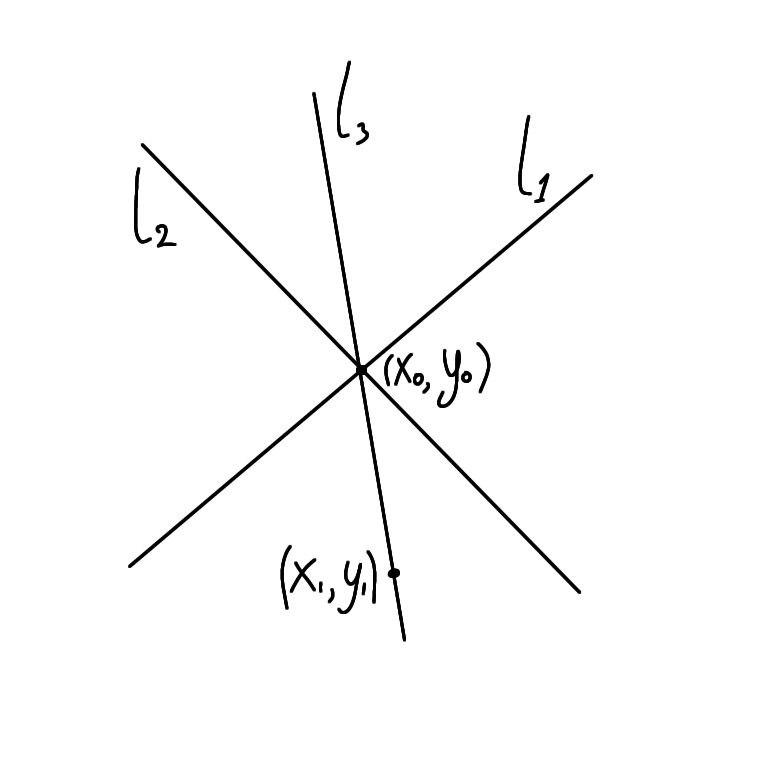
\includegraphics[width=0.84\linewidth]{images/1.5.jpeg}
\end{wrapfigure}

\tab\\

\begin{proof}
    Возьмем на $l_3$ точку ($x_1$, $y_1$), отличную от ($x_0$, $y_0$).
    Тогда
    \[
    (A_2 x_1 + B_2 y_1 + C_2)(A_1 x_1 + B_1 y_1 + C_1) - (A_1 x + B_1 y + C_1)(A_2 x + B_2 y + C_2) = 0,
    \]
    где $(A_2 x_1 + B_2 y_1 + C_2)$ = $\alpha$, $(-(A_1 x + B_1 y + C_1))$ = $\beta$ $\Longrightarrow$ $\alpha^2 + \beta^2 > 0$, т.к. ($x_1$, $y_1$) $\neq$ ($x_0$, $y_0$), но при этом ($x_1$, $y_1$) и ($x_0$, $y_0$) удовлетворяют этому уравнению.

    Осталось доказать, что полученное уравнение $-$ уравнение прямой, т.е. коэффициенты при x и y не могут одновременно равняться нулю, т.е.
    \[
    \left[
        \begin{gathered}
            \alpha A_1 + \beta A_2 \neq 0\\
            \alpha B_1 + \beta B_2 \neq 0\\
        \end{gathered}
    \right.
    \]
    Рассмотрим противное.
    $\begin{vmatrix}
        A_1 & A_2\\
        B_1 & B_2\\
    \end{vmatrix}$ $\neq$ 0, т.к. прямые различны $\Longrightarrow$ система имеет единственное решение при $\alpha$ = $\beta$ = 0 $\Longrightarrow$ противоречие
\end{proof}
\section{Плоскости в пространстве}

\subsection{Векторное параметрическое уравнение плоскости}

Пусть задана система координат O, $\overline{e_1}$, $\overline{e_2}$, $\overline{e_3}$.

\begin{wrapfigure}{l}{0.4\textwidth}
    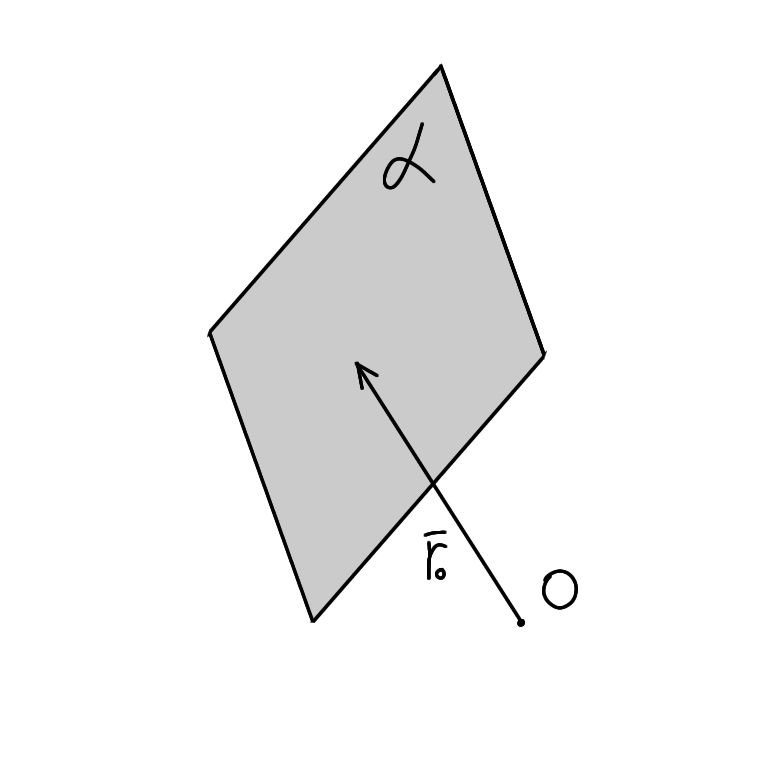
\includegraphics[width=0.84\linewidth]{images/2.1.jpeg}
\end{wrapfigure}

$\alpha$ $-$ плоскость в этой системе координат.\\

$\overline{p}$, $\overline{q}$ $-$ неколлинеарные и параллельные $\alpha$ вектора.\\

\underline{Векторное параметрическое уравнение плоскости}
\[
\overline{r} = \overline{r_0} + t_1\overline{p} + t_2\overline{q},\tab t_1, t_2\in\R
\]
\[
\begin{pmatrix}
    x\\
    y\\
    z\\
\end{pmatrix} = 
\begin{pmatrix}
    x_0\\
    y_0\\
    z_0\\
\end{pmatrix} + 
\begin{pmatrix}
    p_x\\
    p_y\\
    p_z\\
\end{pmatrix}t_1 + 
\begin{pmatrix}
    q_x\\
    q_y\\
    q_z\\
\end{pmatrix}t_2
\]
\tab\\

\subsection{Общее уравнение плоскости}

Заметим, что точка принадлежит плоскости $\Longleftrightarrow$ $\overline{r} - \overline{r_0}$, $\overline{p}$, $\overline{q}$ $-$ компланарны, т.е. ($\overline{r} - \overline{r_0}, \overline{p}, \overline{q}$) = 0 $\Longrightarrow$

\[
\begin{vmatrix}
    x - x_0 & y - y_0 & z - z_0\\
    p_x & p_y & p_z\\
    q_x & q_y & q_z\\
\end{vmatrix} = 0
\]
\[
\Longrightarrow 
\begin{vmatrix}
    p_y & p_z\\
    q_y & q_z\\
\end{vmatrix}(x - x_0) + 
\begin{vmatrix}
    p_x & p_z\\
    q_x & q_z\\
\end{vmatrix}(y - y_0) +
\begin{vmatrix}
    p_x & p_y\\
    q_x & q_y\\
\end{vmatrix}(z - z_0) = 0
\]

Таким образом, получили \underline{общее уравнение плоскости}

\[
\begin{cases}
    Ax + By + Cz + D = 0\\
    A^2 + B^2 + C^2 > 0 (\text{т.к. $\overline{p}$ и $\overline{q}$ - неколлинеарные})
\end{cases}
\]

\begin{theorem}
    Пусть в любой системе координат заданы общее уравнение плоскости Ax + By + Cz + D = 0 и вектор $\overline{a}(\alpha, \beta, \gamma)$ (возможен случай $\overline{a} = \overline{0}$).\\

    Тогда $\overline{a}$ параллелен плоскости $\Longleftrightarrow$ $A\alpha + B\beta + C\gamma$ = 0
\end{theorem}

\begin{proof}
    Пусть $\overline{r_0}(x_0, y_0, z_0)\in$плоскости $\Longrightarrow$ 
    \[
    Ax_0 + By_0 + Cz_0 + D = 0\eqno{(1)}
    \]

    $\overline{a}$ параллельно плоскости $\Longleftrightarrow$ $\overline{r_0} + \overline{a}$ принадлежит плоскости $\Longleftrightarrow$
    \[
    A(x_0 + \alpha) + B(y_0 + \beta) + C(z_0 + \gamma) + D = 0\eqno{(2)}
    \]

    Вычитая (1) из (2), получим $A\alpha + B\beta + C\gamma$ = 0
\end{proof}

\begin{corollary}
    Если задано уравнение вида Ax + By + Cz + D = 0 ($A^2 + B^2 + C^2 > 0$), то оно задает плоскость.
\end{corollary}
\begin{proof}
    Мы можем переписать уравнение в следующем виде

    \begin{itemize}
        \item При C $\neq$ 0:
        \[
        \begin{vmatrix}
            x + \dfrac{DA}{A^2 + B^2 + C^2} & y + \dfrac{DB}{A^2 + B^2 + C^2} & z + \dfrac{DC}{A^2 + B^2 + C^2}\\
            0 & -C & B\\
            C & 0 & -A\\
        \end{vmatrix} = 0
        \]
        где $\overline{p}$ = (0, -C, B) и $\overline{q}$ = (C, 0, -A) $-$ неколлинеарные вектора $\Longrightarrow$ уравнение задает плоскость.

        \item При С = 0:
        \[
        \begin{vmatrix}
            x + \dfrac{DA}{A^2 + B^2} & y + \dfrac{DB}{A^2 + B^2} & z + 0\\
            -B & A & 0\\
            0 & 0 & 1\\
        \end{vmatrix} = 0
        \]
        где $\overline{p}$ = (-B, A, 0) и $\overline{q}$ = (0, 0, 1) $-$ неколлинеарные вектора $\Longrightarrow$ уравнение задает плоскость.
    \end{itemize}
\end{proof}

\begin{theorem}
    Пусть плоскости П$_1$ и П$_2$ заданы следующими уравнениями
    \[
    A_1x + B_1y + C_1z + D_1 = 0\\
    A_2x + B_2y + C_2z + D_2 = 0\\
    \]
    Тогда П$_1$ параллельна П$_2$ $\Longleftrightarrow$ $\exists\lambda\neq 0 : A_1 = \lambda A_2$, $B_1 = \lambda B_2$, $C_1 = \lambda C_2$, $D_1 = \lambda D_2$
\end{theorem}

\subsection{Уравнение плоскости через 3 точки}

Пусть $\overline{r_1}(x_1, y_1, z_1)$, $\overline{r_2}(x_2, y_2, z_2)$, $\overline{r_3}(x_3, y_3, z_3)$ не лежат на одной прямой. Тогда
\[
\overline{r} = \overline{r_1} + t_1(\overline{r_2} - \overline{r_1}) + t_2(\overline{r_3} - \overline{r_1})
\]
\[
\begin{vmatrix}
    x - x_1 & y - y_1 & z - z_1\\
    x_2 - x_1 & y_2 - y_1 & z_2 - z_1\\
    x_3 - x_1 & y_3 - y_1 & z_3 - z_1\\
\end{vmatrix} = 0
\]
\clearpage
\subsection{Уравнение плоскости через нормальный вектор}

\begin{wrapfigure}{l}{0.4\textwidth}
    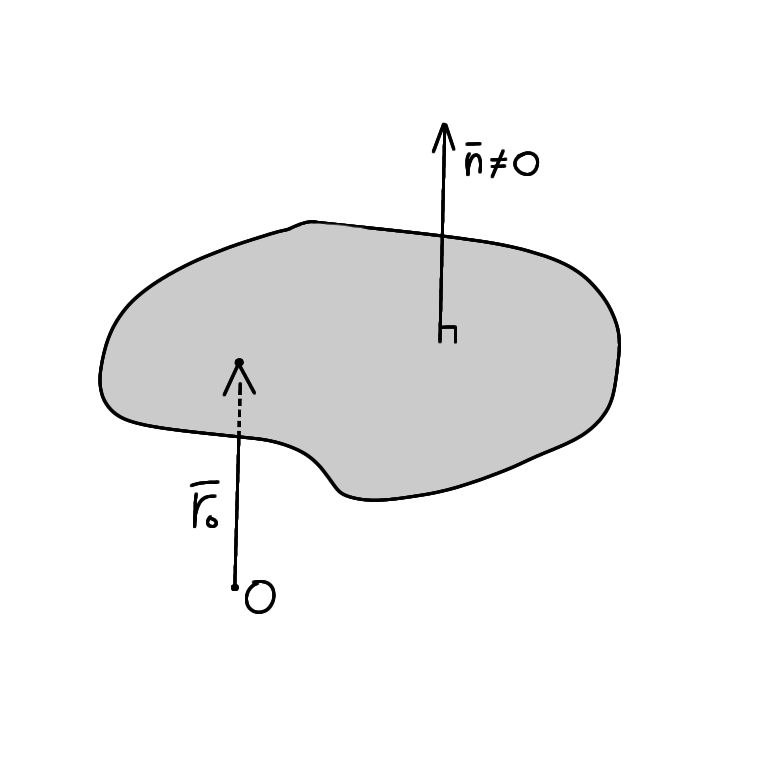
\includegraphics[width=0.84\linewidth]{images/2.2.jpeg}
\end{wrapfigure}

\tab\\

Пусть заданы точка $\overline{r_0}$, принадлежащая плоскости, и нормальный вектор $\overline{n}$. Тогда
\[
(\overline{r} - \overline{r_0}) = 0, \tab (\overline{r}, \overline{n}) = d
\]

В ОНБ один из способов задать нормалный вектор $\overline{n}$ = (A, B, C).

\tab\\ \tab\\ \tab\\ \tab\\
\subsection{Расстояние от точки до плоскости}

\underline{В произвольной системе координат.}\\

Пусть заданы точка $M_0$($\overline{r_1}$) и плоскость ($\overline{r} - \overline{r_0}$, $\overline{n}$) = 0. Тогда расстояние от $M_0$ до плоскости
\[
\rho = \dfrac{|(\overline{r_1} - \overline{r_0}, \overline{n})|}{|\overline{n}|}
\]

\underline{В ОНБ.}\\

\[
\overline{n}(A, B, C), M(x_1, y_1, z_1), Ax + By + Cz + D = 0 \Longrightarrow
\]
\[
\rho = \dfrac{|Ax_1 + By_1 + Cz_1 + D|}{\sqrt{A^2 + B^2 + C^2}}
\]
\subsection{Пучок плоскостей}

\begin{definition}
    \textit{Пучок плоскостей} $-$ множество плоскостей, проходящих через одну прямую.
\end{definition}

\begin{definition}
    \textit{Связка плоскостей} $-$ множество плоскостей, проходящих через одну точку.
\end{definition}
\clearpage
\section{Прямые в пространстве}

\subsection{Способы задания прямой в пространстве}

\underline{Каноническое уравнение прямой}\\

\begin{wrapfigure}{l}{0.3\textwidth}
    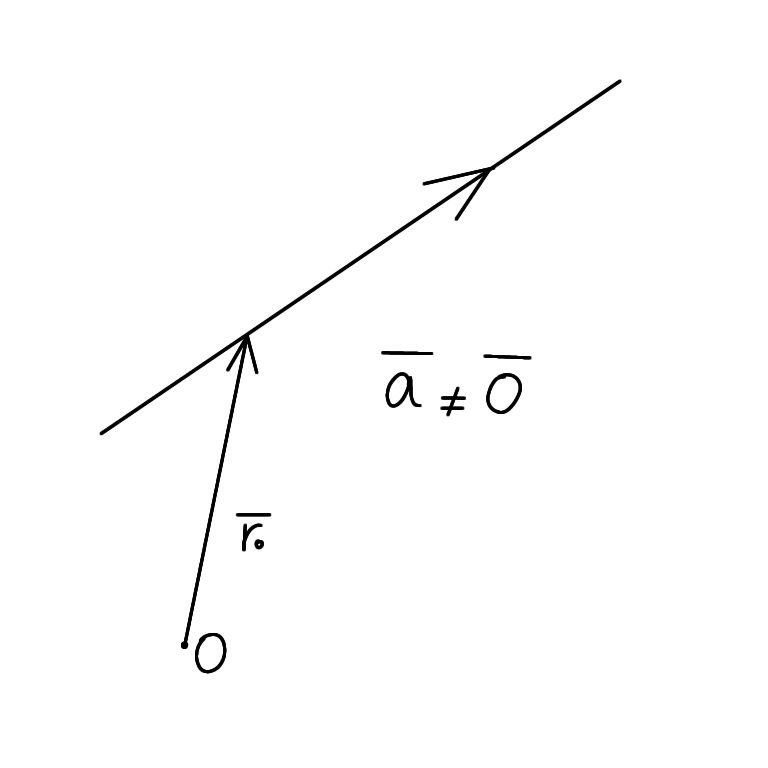
\includegraphics[width=0.84\linewidth]{images/3.1.jpeg}
\end{wrapfigure}

\tab\\

\[
\begin{cases}
    \overline{r} = \overline{r_0} + \overline{a}t\\
    x = x_0 + a_xt\\
    y = y_0 + a_yt\\
    z = z_0 + a_zt\\
\end{cases} 
\]
\[
\Longrightarrow \tab \dfrac{x - x_0}{a_x} = \dfrac{y - y_0}{a_y} = \dfrac{z - z_0}{a_z}
\]
\tab\\
\underline{Через пару точек $\overline{r_1}$ и $\overline{r_2}$}\\

\[
\overline{r} = \overline{r_1} + t(\overline{r_2} - \overline{r_1})
\]
\[
\Longleftrightarrow
\]
\[
\dfrac{x - x_1}{x_2 - x_1} = \dfrac{y - y_1}{y_2 - y_1} = \dfrac{z - z_1}{z_2 - z_1}
\]

\underline{Через направляющий вектор}\\

\[
[\overline{r} - \overline{r_0}, \overline{a}] = \overline{0}\\
\]
\[
[\overline{r}, \overline{a}] = \overline{d}
\]

\underline{Через две плоскости}\\

Пусть заданы две плоскости П$_1$ и П$_2$, тогда прямая $-$ пересечение этих плоскостей.

\subsection{Углы между прямыми и плоскостями}

\begin{definition}
    Углом между плоскостями ($\overline{r} - \overline{r_{01}}, \overline{n_1}$) = 0 и ($\overline{r} - \overline{r_{02}}, \overline{n_2}$) = 0 называется угол между их нормальными векторами $\overline{n_1}$ и $\overline{n_2}$.
\end{definition}

\begin{definition}
    Углом между плоскостью ($\overline{r} - \overline{r_{0}}, \overline{n}$) = 0 и прямой $\overline{r}$ = $\overline{r_0} + t\overline{a}$ называется угол $\dfrac{\pi}{2} - \alpha$, где $\alpha$ - угол между векторами $\overline{n}$ и $\overline{a}$.
\end{definition}

\subsection{Расстояния между точками, прямыми и плоскостями в пространстве}

\underline{Расстояние от точки до прямой в пространстве}\\

\begin{wrapfigure}{l}{0.3\textwidth}
    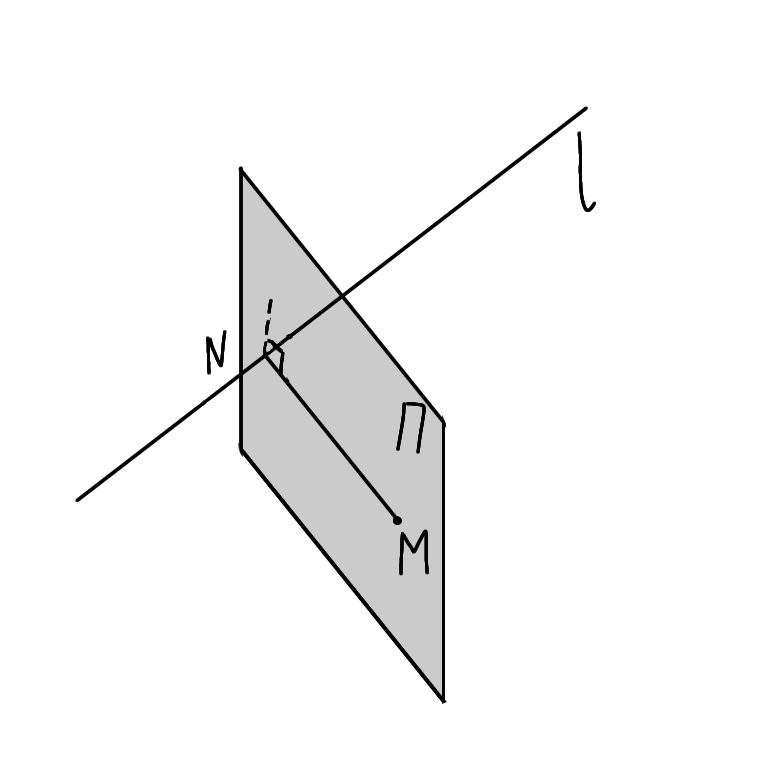
\includegraphics[width=0.84\linewidth]{images/3.2.jpeg}
\end{wrapfigure}
\tab\\

    1 способ. Проведем плоскость П, которая проходит через точку М перпендикулярно прямой l. Тогда
    \[
    \rho = \rho(M, N)
    \]

    \tab\\ \tab\\ \tab\\ \tab\\ \tab\\

\begin{wrapfigure}{l}{0.3\textwidth}
    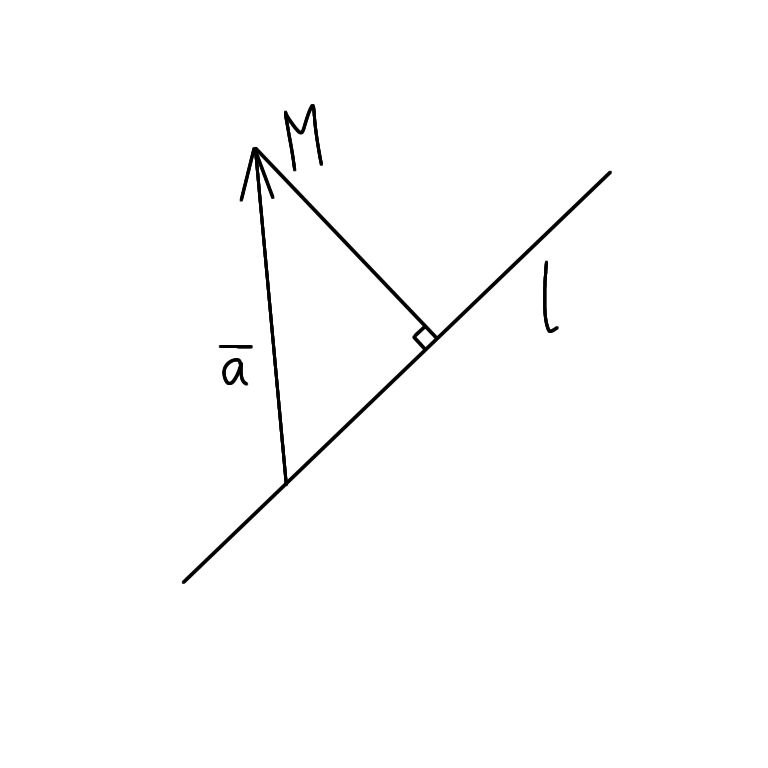
\includegraphics[width=0.84\linewidth]{images/3.3.jpeg}
\end{wrapfigure}
\tab\\

    2 способ. Спроецируем $\overline{a}$ на прямую l и найдем ортогональную составляющую $-$ искомое расстояние.

    \tab\\ \tab\\ \tab\\ \tab\\ \tab\\ \tab\\ \tab\\

\begin{wrapfigure}{l}{0.3\textwidth}
    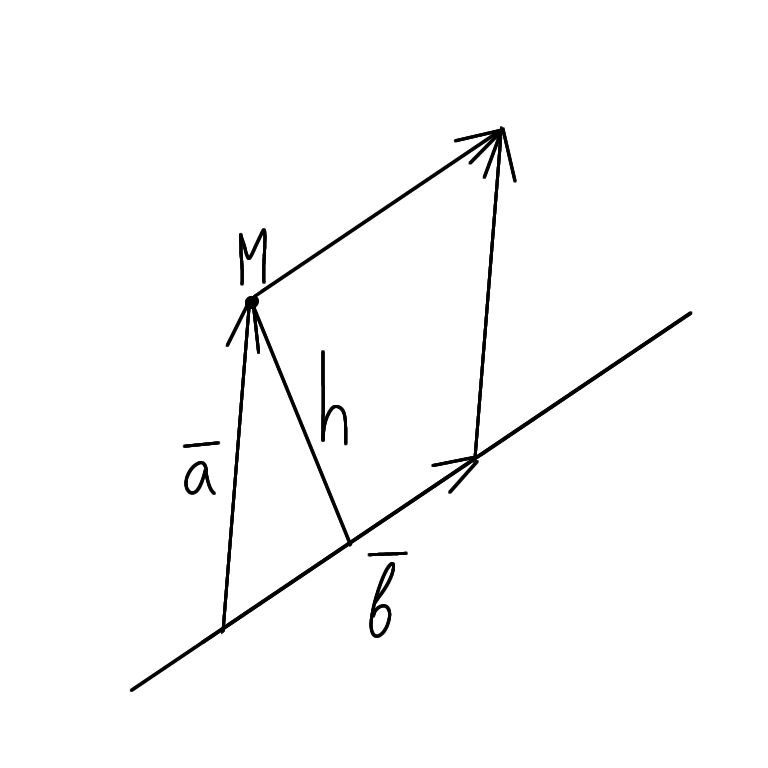
\includegraphics[width=0.84\linewidth]{images/3.4.jpeg}
\end{wrapfigure}
\tab\\

    3 способ. \[
    \rho = \dfrac{S\mkern-2mu{\rotatebox{-60}{\(\lozenge\)}}}{|\overline{b}|} = \dfrac{|[\overline{a}, \overline{b}]|}{|\overline{b}|}
    \]

    \tab\\ \tab\\ \tab\\ \tab\\ \tab\\
\underline{Расстояние между прямыми в пространстве}\\

Пусть заданы две прямые $l_1$ и $l_2$.\\

Если $l_1$ || $l_2$, то расстояние от любой точки $l_1$ до $l_2$ $-$ искомое.\\

Если $l_1$ и $l_2$ $-$ скрещивающиеся (возможно пересечение), то\\

\begin{wrapfigure}{l}{0.3\textwidth}
    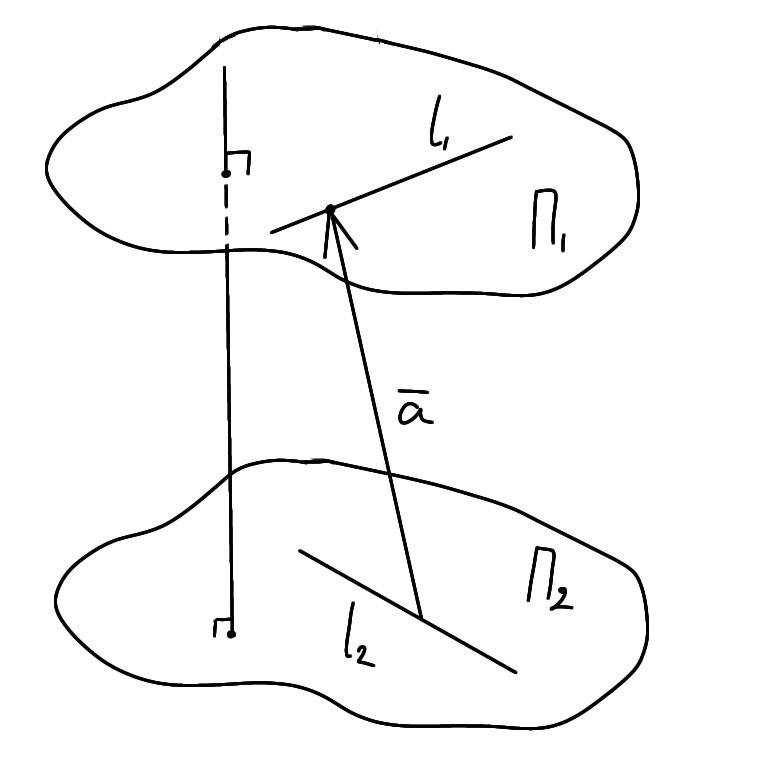
\includegraphics[width=0.84\linewidth]{images/3.6.jpeg}
\end{wrapfigure}

\tab\\

1 способ. Проведем плоскость через $l_1$ параллельно $l_2$  и посчитаем расстояние от точки на $l_2$  до плоскости.\\

2 способ. Проведем через прямые параллельные плоскости, а к ним проведем общий перпендикуляр, тогда искомое расстояние $-$ скалярная проекция $\overline{a}$ на него.\\

3 способ. \[
\rho = \dfrac{|(\overline{a}, \overline{b}, \overline{c})|}{|[\overline{a}, \overline{b}]|}
\]
\section{Алгебраические линии и поверхности}

В пространстве рассмотрим уравнения вида
\[
A_1 x^{\alpha_1}y^{\beta_1}z^{\gamma_1} + A_2 x^{\alpha_2}y^{\beta_2}z^{\gamma_2} + ... + A_k x^{\alpha_k}y^{\beta_k}z^{\gamma_k} = 0,\tab \alpha_i, \beta_i, \gamma_i \in \Z \geq 0
\]

\begin{definition}
    \textit{Степень уравнения}, или \textit{порядок алгебраической поверхности} $-$
    \[
    T = \underset{i=1..k}{max}(\alpha_i + \beta_i + \gamma_i)
    \]

    Аналогично на плоскости задается алгебраическая линия порядка T = $\underset{i=1..k}{max}(\alpha_i + \beta_i)$
\end{definition}

\begin{theorem}
    Алгебраическая поверхность(линия) порядка p в любой системе координат может быть задана уравнением порядка p.
\end{theorem}
\begin{proof}
    \[
    \begin{cases}
        x = a_{11}x' + a_{12}y' + a_{13}z'\\
        y = a_{21}x' + a_{22}y' + a_{23}z'\\
        z = a_{31}x' + a_{32}y' + a_{33}z'\\
    \end{cases}
    \]
    Подставив полученные координаты в уравнение, получим, что максимальная степень m такая, что порядок не увеличится.

    Заметим также, что если порядок уменьшится, то при обратной замене он должен увеличиться, значит получим противоречие $\Longrightarrow$ порядок не изменился.
\end{proof}

\begin{lemma}
    Пусть существует алгебраическая поверхность(линия) порядка n. Тогда прямая и алгебраическая поверхность(линия) могут иметь 0, 1, ..., n или бесконечно много общих точек.
\end{lemma}

